%%%%%%%%%%%%%%%%%%%%%%%%%%%%%%%%%%%%%%%%%%%%%%%%%%%%%%%
%% Bachelor's & Master's Thesis Template             %%
%% Copyleft by Artur M. Brodzki & Piotr Woźniak      %%
%% Faculty of Electronics and Information Technology %%
%% Warsaw University of Technology, 2019-2020        %%
%%%%%%%%%%%%%%%%%%%%%%%%%%%%%%%%%%%%%%%%%%%%%%%%%%%%%%%

\documentclass[
    left=2.5cm,         % Sadly, generic margin parameter
    right=2.5cm,        % doesnt't work, as it is
    top=2.5cm,          % superseded by more specific
    bottom=3cm,         % left...bottom parameters.
    bindingoffset=6mm,  % Optional binding offset.
    nohyphenation=false % You may turn off hyphenation, if don't like.
]{eiti/eiti-thesis}
\langpol % Dla języka angielskiego mamy \langeng
\graphicspath{{img/}}             % Katalog z obrazkami.
\addbibresource{bibliografia.bib} % Plik .bib z bibliografią

\begin{document}

%--------------------------------------
% Strona tytułowa
%--------------------------------------
\MasterThesis % Dla pracy inżynierskiej mamy \EngineerThesis
\instytut{XXXXXX}
\kierunek{XXXXXX}
\specjalnosc{XXXXXX}
\title{
    Niepotrzebnie długi i skomplikowany tytuł pracy \\
    trudny do przeczytania, zrozumienia i wymówienia
}
\engtitle{ % Tytuł po angielsku do angielskiego streszczenia
    Unnecessarily long and complicated thesis' title \\
    difficult to read, understand and pronounce
}
\author{\{Imię i Nazwisko\}}
\album{XXXXXX}
\promotor{XXXXXX}
\date{\the\year}
\maketitle

%--------------------------------------
% Streszczenie po polsku
%--------------------------------------
\cleardoublepage % Zaczynamy od nieparzystej strony
\streszczenie \lipsum[1-3]
\slowakluczowe XXX, XXX, XXX

%--------------------------------------
% Streszczenie po angielsku
%--------------------------------------
\newpage
\abstract \kant[1-3]
\keywords XXX, XXX, XXX

%--------------------------------------
% Oświadczenie o autorstwie
%--------------------------------------
\cleardoublepage  % Zaczynamy od nieparzystej strony
\pagestyle{plain}
\makeauthorship

%--------------------------------------
% Spis treści
%--------------------------------------
\cleardoublepage % Zaczynamy od nieparzystej strony
\tableofcontents

%--------------------------------------
% Rozdziały
%--------------------------------------
\cleardoublepage % Zaczynamy od nieparzystej strony
\pagestyle{headings}

\newpage % Rozdziały zaczynamy od nowej strony.
\section{Wstęp}
Kwestia wiarygodności informacji napływających do nas ze wszystkich mediów stała się ostatnio gorącym tematem. Mimo faktu, że problem występuje od zawsze, w\,ostatnich latach zwrócił na siebie dużo uwagi. Przy ilości informacji jaka jest udostępniana w Internecie, w\,szczególności dzięki możliwości udostępniania wszystkiego poprzez portale społecznościowe, szerzenie dezinformacji stało się bardzo proste i\,szybkie. Mogą one przyjmować rozmaitą formę zaczynając na krótkiej formie tekstowej jaką są Tweety, poprzez kłamliwe artykuły naukowe, przerobione zdjęcia na zmanipulowanych filmach wideo kończąc. Należy więc podjąć próbę wykrycia prawdziwości pojawiających się treści. Można to wykonać przez pracę człowieka lub automatycznie.
\par
W ostatnich latach powstaje coraz więcej inicjatyw próbujących zrozumieć i\,powstrzy- mać to zjawisko skupiając się zarówno na podłożu socjologicznym jak również tworząc nowe rozwiązania informatyczne których zadaniem będzie pomoc użytkownikom w\,rozróżnieniu prawdy od dezinformacji. Takich projektów jednak jest nadal bardzo mało i\,w\,większości nie obejmują one innych języków niż angielski.
\par
W poniższej pracy przedstawiono opis problemu jakim są nierzetelne informacje oraz zebrano dotychczasowe rozwiązania oceny prawdziwości treści. Następnie opracowano badania porównujące cechy kont oraz publikowanych treści w\,mediach społecznościowych. Badano treści w\,języku polskim oraz porównywano konta zakwalifikowane jako nierzetelne do kont określanych jako wiarygodne. Takiego podziału dokonano na podstawie kilku niezależnych źródeł. Na podstawie zebranych danych dokonano badania automatycznej klasyfikacji treści pochodzących z\,portalu społecznościowego na podstawie ich kontekstu. Klasyfikowano czy post należy do klasy nierzetelnych czy też nie wykorzystując wiedzę jego odbiorcach.
\par
Na wstępie przeprowadzono rozpoznanie problemu, czynniki mu sprzyjające oraz jego wpływ na rzeczywistość. Następnie na podstawie dostępnej literatury i\,istniejących badań przedstawiono najbardziej popularne sposoby rozwiązania problemu klasyfikacji informacji pod względem ich wiarygodności. 
\par
Okazuje się, że większość istniejących projektów w\,tym temacie skupia się wyłącznie na tematyce polityki w\,USA. Jedynie pojedyncze zespoły podjęły do tej pory działania obejmujące obszary związane z\,innymi językami niż angielski oraz inną strefą tematyczną. Według najlepszej wiedzy autora, nie istnieją w\,tym momencie żadne inicjatywy podejmujące temat klasyfikacji informacji w\,mediach społecznościowych w\,języku polskim. Z tego powodu poniższa praca w\,dalszej swojej części skupia się na rozpoznaniu problemu wiarygodności informacji w\,polskiej przestrzeni internetowej. Przytoczone zostaną badania opinii społecznej oraz zanalizowane zostaną dostępne badania obejmujące tematy Unii Europejskiej. 
\par
W drugiej części pracy zostanie przeprowadzona oraz opisana analiza wybranych danych pochodzących z\,polskojęzycznych postów opublikowanych w mediach społecznościowych. Celem tej analizy będzie znalezienie właściwości i\,charakterystyk kont uznanych za nierzetelne. W\,celu analizy porównawczej konta te zostaną przeciwstawione kontom należącym do profesjonalnych serwisów informacyjnych, serwisów o dużej liczbie odsłon oraz portali specjalizujących w sprawdzaniu prawdziwości innych mediów (tzw.\,factchecking).
\par
Ostatnim badaniem przeprowadzonym w\,ramach tej pracy będzie dokonanie próby automatycznej klasyfikacji treści pochodzących z\,mediów społecznościowych na podstawie ich kontekstu. Kontekstem, który zostanie przyjęty będzie interakcja użytkowników portalu z\,badanymi treściami. Celem tego badania jest sprawdzenie możliwości wykonania takiej klasyfikacji i\,jej precyzji. Dodatkowo zostanie zbadane jak duża musi być zaklasyfikowana próbka treningowa, aby otrzymać zadowalające wyniki klasyfikacji. Do wykonania tej klasyfikacji zostaną użyte dwa algorytmy. Pierwszym z\,nich jest klasyczny algorytm uczenia maszynowego jakim jest regresja logistyczna, a\,drugim będzie zastosowanie algorytmu etykietowania przez użytkowników używając właściwości rozprzestrzeniania wiedzy w\,sieci. 
\par
Na koniec podsumowana zostanie cała zdobyta wiedza oraz wyniki przeprowadzonych badań. Zostaną zebrane wnioski oraz wynikająca z\,nich nauka dla przyszłych inicjatyw chcących badać lub automatycznie wykrywać nieprawdziwe informacje publikowane za pomocą mediów społecznościowych. 

  

\newpage % Rozdziały zaczynamy od nowej strony.
\section{Podjęta problematyka}
Zjawisko intencjonalnego publikowania nieprawdziwych informacji dostało nazwę fake news. 
Ten neologizm został również zaadoptowany w\,języku polskim. Słownik języka polskiego PWN w\,dziale ciekawostki definiuje zwrot fake news jako „nieprawdziwe, fałszywe wiadomości, najczęściej rozpowszechniane przez tabloidy w\,celu wywołania sensacji, bądź zniesławienia kogoś (najczęściej polityka)”. Według językoznawcy nie jest to w\,języku polskim już tylko słowo slangowe, jako że wygrało w\,plebiscycie słowników Collinsa w\,roku 2017\footnote{\url{https://sjp.pwn.pl/ciekawostki/haslo/fake-news;6368870.html}}.  Inaczej możemy to zjawisko nazywać dezinformacją, które jest definiowana jako „fałszywa, rzekoma informacja, zamierzone wprowadzenie w\,błąd” \footnote{\url{https://sjp.pl/dezinformacja}}. 
Może ono objawiać się pod różnymi formami, najbardziej kojarzą się z\,ich pierwotną formą jaką są artykuły w\,mediach szerzące nieprawdę. Mimo że ten problem występuje tak długo jak istnieją media obecnie jednak jego wpływ jest dużo większy. 

\subsection{Problematyka nierzetelnych informacji}
Szerzenie się nieprawdziwych, nierzetelnych informacji w\,mediach, z\,których pobieramy wiedzę o świecie nie może być ignorowane. Wielkość tego zjawiska już teraz stwarza dużo problemów i \,ciągle się powiększa. Coraz więcej osób pobiera najświeższe informacje o wydarzeniach z\,internetu. Informacje można te podzielić ze względu na źródło z\,jakiego pochodzą. Mogą być one bowiem publikowane przez tradycyjne media znane z\,formy papierowej lub telewizyjnej posiadające własną stronę internetową. Ale internet daje również duże możliwości publikowania własnych treści wszystkim użytkownikom, dzieje się to głównie poprzez blogi i\,portale społecznościowe.  \par
Nierzetelne informacje w\,Internecie są poważnym problemem. 68\% Europejczyków natrafia na informacje, które zakłamują rzeczywistość przynajmniej raz w\,tygodniu a\,połowa z\,nich nawet codziennie \cite{Eurobarometer4642018}. Na szczęście 71\% z\,nich twierdzi, że jest raczej pewnych w\,swoich umiejętnościach wykrycia czy czytana przez nich informacja o wydarzeniach jest prawdziwa czy też nie. Mimo to nierzetelne informacje występują w\,mediach społecznościowych a\,użytkownicy często wchodzą z\,nimi w\,interakcje poprzez udostępnianie ich dalej.
\par Mimo tego, że więcej użytkowników Internetu nadal bardziej ufa źródłom związanym z\,tradycyjnymi mediami niż informacjom generowanym przez użytkowników \cite{rieh2014credibility} to według badań z\,2018 roku 68 procent ankietowanych amerykanów zadeklarowało, że zdarza im się czytać informacje za pomocą portali społecznościowych \cite{PewNewsUse2018}. Takie badania co roku przeprowadza Centrum Badań Pew. Według ich danych wzrost liczby osób korzystających z\,portali społecznościowych do zdobywania wiadomości o świecie w\,ostatnim roku przystopowała po czasie dużego wzrostu w\,poprzednich latach.

\subsubsection{Social media}
Widać, więc jak duże jest nadal znaczenie portali społecznościowych w\,szerzeniu informacji. Dzieje się tak z\,kilku powodów. Dla użytkowników jest to po prostu wygodne. Przeglądając główną stronę aplikacji użytkownik dostaje posty subskrybowanych przez siebie stron informacyjnych lub posty z\,którymi weszli w\,interakcje jego znajomi. Dzieje się tak w\,szczególności dla portalu Facebook, gdzie większość użytkowników spotyka posty informacyjne robiąc inne rzeczy na portalu a \,nie szukając ich specjalnie \cite{PewNewsUse2016}. Takie pobieranie informacji nie wymaga od użytkownika większego wysiłku a\,daje duże możliwości. Są one świetnym źródłem informacji o najświeższych wydarzeniach jak również relacji naocznych świadków wydarzeń lub wypowiedzi osób bezpośrednio z\,nimi związanych. Użytkownik dodatkowo może wchodzić w\,interakcję z\,innymi odbiorcami. W\,łatwy sposób może komentować i \,uczestniczyć w\,dyskusji na wybrane przez siebie tematy. Popularność portali społecznościowych wykorzystują więc wszystkie instytucje, które chcą przekazać informację lub swoją opinię. Krótkie notki publikowane na takich portalach mogą powstawać szybko i \,małym kosztem w\,porównaniu do pełnowymiarowego artykułu. 
\par Niestety wszystkie wymienione wyżej czynniki tworzą doskonałe podłoże do szerzenia dezinformacji. Każdy może napisać cokolwiek chce. Świeże posty bardzo ciężko jest zweryfikować pod względem prawdziwości a \,mogą szybko zostać rozniesione między użytkownikami serwisu. Głównym problemem w\,rozprzestrzenianiu dezinformacji lub treści o tematyce konspiracyjnej mogą być sami użytkownicy. Badania wykazały, że posty publikowane przez strony zakwalifikowane jako konspiracyjne otrzymują więcej ‘polubień’ oraz udostępnień przez użytkowników niż posty publikowane przez portale naukowe \cite{bessi2015science}. 

\subsection{Powody popularności Fake News}
Należy się zastanowić, dlaczego w\,ogóle część użytkowników preferuje przyjmowanie wiadomości, które nie są prawdziwe. Można by założyć, że większość społeczeństwa nie akceptuje bycia okłamywanym. Dlaczego więc jakaś grupa toleruje otaczające go fałszywe informacje.  Problem ten nie występuje tylko w\,oparciu o\,informacje przekazywane przez media społecznościowe, ale również media tradycyjne takie jak czasopisma, radio i\,telewizja. 
\par Powody, dla których poddajemy się przyjmowaniu fałszywych informacji możemy podzielić na dwa rodzaje: psychologiczne i \,społeczne \cite{shu2017fake}. Te pierwsze są w\,szczególności wykorzystywane przez media tradycyjne, które samemu wybieramy, natomiast społeczne są wyjątkowo nasilone, jeśli mamy możliwość lub musimy wyrazić głośno swoją opinię.

\subsubsection{Czynniki psychologiczne}
Psychologiczne powody sięgania po określone treści mogą być spowodowane zjawiskiem nazwanym naiwnym realizmem. Polega ono na tym, że człowiek sądzi, że to co on wie lub w\,co wierzy jest jedyną prawdą, a\,jeśli się koś z\,nim nie zgadza to musi być niedoinformowany lub nieracjonalny. Jest to powiązane z\,efektem potwierdzenia. Jest to zjawisko w\,psychologii, gdzie człowiek zawsze będzie wybierał informacje, które potwierdzają jego wcześniej utarte przekonania. Prowadzi to również do selektywnego wybierania dowodów oraz interpretowania ich na korzyść swoich przekonań.  Występuje to w\,szczególności przy tematach, którym towarzyszą skrajne opinie i \,duże emocje. Przy tym często taka opinia jest oparta na pierwszych informacjach, które przyswoił. Dlatego ludzie czasem sięgają po konkretne informacje nie zważając na ich prawdziwość.  Dodatkowo bardzo trudno jest zmienić zdanie takiej osoby. Przedstawianie im treści, która naprostowuje nierzetelne informacje często nie daje żadnych efektów lub wręcz pogłębia ich wcześniejszą opinię. 

\subsubsection{Czynniki społeczne}
Człowiek jest istotą społeczną, można więc powiedzieć, że jedną z\,jego głównych potrzeb jest przynależność do grupy i \,bycie akceptowanym przez innych. Jest to nawet zaznaczone w\,modelu hierarchii potrzeb Maslowa. Ta podświadoma potrzeba może objawiać się w\,taki sposób, że osobnik będzie wyrażał opinię, która jest popularna w\,jego otoczeniu. Oznacza to zarówno, że będzie preferował odbieranie informacji, które nawiązują do przekonań jego grupy. Może się to utrzymać również w\,sytuacji, kiedy te informacje są spaczone lub stronnicze. Mimo to dla osobnika będzie to wybór społecznie bezpieczny.

\subsection{Efekt komory pogłosowej}
Media społecznościowe dają jeszcze większe możliwości przyjmowania informacji, wyrażania głośno swojej aprobaty i \,emocji jakie wywołują oraz dyskusji na ich temat z\,innymi użytkownikami. Dodatkowo można w\,łatwy sposób wybierać preferowane źródła, które publikują preferowane przez nas tematy lub opinie. Mimo wielu zalet takich jak wygoda w\,otrzymywaniu interesujących nas wiadomości i \,ciekawostek może to tworzyć efekt komory pogłosowej (ang. echo chamber effect) \cite{garimella2018political}. Charakteryzuje się on zjawiskiem, że użytkownik na portalu społecznościowym otacza się znajomymi o podobnych do siebie poglądach oraz subskrybuje kanały publikujące informacje, które uznaje za ciekawe, często takie z\,których opinią się zgadza. Dodatkowo najczęściej wykazuje aktywność poprzez dodanie reakcji do postu, udostępnienie go w\,przypadku treści z\,którymi zdecydowanie się zgadza lub budzą w\,nim duże emocje. Takie działania dają informację algorytmom portali na temat preferowanych przez użytkownika postów. Takie algorytmy stworzone są w\,celu zwiększenia ruchu na portalu co jest wykonywane między innymi przez zwiększenie satysfakcji użytkownika z\,otrzymywanych treści.  Algorytm wybiera więc posty odpowiadające stworzonym warunkom dla poszczególnego użytkownika. Takim sposobem tworzy się bańka komory pogłosowej. Użytkownik i \,osoby o podobnych opiniach będą otrzymywały pasujące dla nich treści. 
\par To zjawisko może być użyte do szerzenia dezinformacji. Pomagają temu dodatkowe czynniki wpływające na użytkownika  \cite{shu2017fake}. Pierwszą z\,nich jest wiarygodność społeczna, która polega na założeniu, że im więcej osób uznaje informację, lub całe źródło informacji za wiarygodne tym bardziej prawdopodobne, że inni również uznają ją za wiarygodne. W\,mediach społecznościowych jest to powiązane ze zjawiskiem heurystyki dostępności, które w\,tym kontekście można przedstawić przy pomocy niesławnego powiedzenia „Kłamstwo powtarzane wiele razy staje się prawdą”. Oznacza to, że jeśli usłyszymy pewną informację wystarczająco dużo razy, tym bardziej prawdopodobne, że uwierzymy w\,jej prawdziwość nawet gdy tak nie jest. Oba te czynniki występują w\,dużej ilości w\,mediach społecznościowych przy tworzących się bańkach komory pogłosowej i \,są bardzo podatne na rozsyłanie dezinformacji w\,taki sposób, aby użytkownicy ją akceptowali lub wręcz w\,nią uwierzyli. 

\subsection{Wpływ na rzeczywistość}
Najbardziej popularnym przykładem roznoszenia fałszywych informacji na dużą skalę jest okres przed wyborami prezydenckimi w\,Stanach Zjednoczonych w\,2016 roku. Zostało stwierdzone, że na portalu Twitter więcej udostępnień zostało wykonanych na postach zawierających fałszywe informacje niż na tych z\,prawdziwymi danymi  \cite{neudertpolarization2018}. Podobne badania przeprowadzono w Unii Europejskiej w czasie poprzedzającym wybory do europarlamentu. W przedstawionych wynikach na rysunku \ref{fig:EUMapJunkNews} wykazano, że w badanych krajach średnia liczba treści z nierzetelnych źródeł to 4\% jednak dla danych polskojęzycznych aż 20\% zebranych treści pochodziło z źródeł uznanych przez ekspertów jako nierzetelne\cite{marchal2019junk}.
\begin{figure}[!h]
	
	\centering 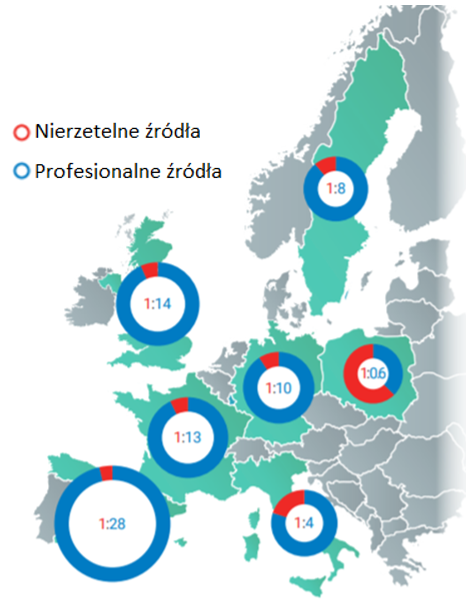
\includegraphics[width=0.5\linewidth]{img/EUMapJunkNews.PNG}
	\caption{Porównanie liczby treści ze źródeł nierzetelnych oraz profesjonalnych w wybranych państwach UE. źródło: \cite{marchal2019junk}}
	\label{fig:EUMapJunkNews}
\end{figure}
\par
Dodatkowo rozsiewanie fałszywych informacji może mieć tak tragiczne skutki jak afera Pizzagate\,\footnote{\url{https://www.nytimes.com/2016/12/05/business/media/comet-ping-pong-pizza-shooting-fake-news-consequences.html}}. Pewien człowiek uwierzywszy w\,teorię spiskową na temat mafii pedofilskiej powiązanej z\,Hillary Clinton wszedł uzbrojony do pizzerii, w\,której miał się odbywać nielegalny proceder i \,otworzył ogień. Na szczęście w\,zajściu nikt nie ucierpiał. Mimo, że przytoczony przykład jest skrajną sytuacją, pokazuje jak łatwo jest manipulować jednostkami. Największy problem pojawia się, jeśli uda się zmanipulować całą masą ludzi. 
\subsection{Podsumowanie problemu}
Fałszywe informacje są często bardzo trudne do wykrycia a\,wciąż rozwijające się algorytmy mogą być używane do szerzenia ich na ogromną skalę. Coraz częściej zaczynamy mówić o problemie wiarygodności w\,dostarczanych nam mediach. Użytkownicy korzystający z\,platform społecznościowych do czytania wiadomości też już zauważyli ten problem. Według najnowszych badań Pew 57\% użytkowników uważa takie informacje za niedokładne \cite{PewNewsUse2018}. Za główne problemy takiego zjawiska wskazują stronniczość polityczną oraz niską jakość publikowanych treści. Nie bez znaczenia jest też zachowanie innych użytkowników. 
\par Żmudne zadanie neutralizacji fałszywych informacji prowadzą już od dawna dedykowane temu portale amerykańskie. W\,polskim Internecie powstał serwis Demagog, który za cel stawia sobie sprawdzanie prawdziwości wypowiedzi polityków. Do walki z\,rozszerzającymi się fałszywymi informacjami włącza się również technologia. Powstaje coraz więcej prób zautomatyzowania wykrywania niewiarygodnych źródeł i\,artykułów mówiących nieprawdę. Automatyczne wykrywanie fake news jest to przewidywanie szans, że konkretny artykuł jest intencjonalnie fałszywy \cite{threeTypeOfFakes2015}. Niestety w\,tak szybko rozwijającym się środowisku jest to zadanie co najmniej trudne. Nie istnieją jeszcze wystarczająco dobre rozwiązania. Należy więc szukać nowych i\,dodatkowo rozszerzać je na inne języki oprócz języka angielskiego. 
       
\newpage % Rozdziały zaczynamy od nowej strony.
\section{Przegląd istniejących rozwiązań klasyfikacji informacji}
W poniższym rozdziale przedstawione zostaną wybrane metody służące do klasyfikacji informacji pod względem zawierania przez nich prawdy lub fałszu. Istnieją dwa główne typy mechanizmów: manualny - wymagający pracy człowieka oraz automatyczny gdzie do klasyfikacji używane są różne typy algorytmów. Automatyczne dodatkowo można wyraźnie rozróżnić pod kątem danych jakie są używane w\,celu klasyfikowania treści. 
\subsection{Rozwiązania manualne}
Do tej grupy zostały zakwalifikowane rozwiązania które w\,dużej mierze lub całkowicie polegają na pracy człowieka. Praca ta polega na manualnej decyzji osoby czy przedstawiony jej tekst zawiera prawdę czy jest dezinformujący. Sposoby tej pracy różnią się zaangażowaniem oceniającej osoby. Jako eksperta traktujemy osobę która poświęca czas i\,posiadaną wiedzę aby poprzeć swoją opinię dowodami z\,wiarygodnych źródeł. Innym sposobem jest użycie tzw. crowdsourcingu który polega na zbieraniu opinii dużej liczby użytkowników, którzy niekoniecznie są całkowicie wiarygodni. 
\subsubsection{Praca ekspertów}
Badanie rzetelności faktów zawartych w\,artykułach lub w\,wypowiedziach osób publicznych jest często zadaniem skomplikowanym oraz czasochłonnym. Są jednak inicjatywy poświęcone wykrywaniu fałszu lub niepełnej prawdziwości w\,publikowanych informacjach. Jednymi z\,najbardziej popularnych stron zajmujących się taką weryfikacją są Politifact\footnote{\url{https://www.politifact.com}} oraz Snopes\footnote{\url{https://www.snopes.com}} . Podejmują one głównie tematy związane ze polityką Stanów Zjednoczonych. Ich działanie polega na zatrudnianiu niezależnych dziennikarzy, których zadaniem jest wyszukiwanie źródeł weryfikujących wiarygodność informacji podawanych w\,sieci. Oceniają oni daną informację według ustalonej klasyfikacji. Aby być samemu być wiarygodnym zawsze podają źródła zarówno sprawdzanej informacji jak i\,materiałów użytych do wydania oceny. Dzięki temu użytkownik sam może zweryfikować swoją opinię. 
\par To rozwiązanie mimo oczywistych plusów, jakimi jest rzetelność i\,przejrzystość weryfikacji wierzytelności ma też znaczące minusy. Wymaga ono dużych nakładów pracy wykonanej przez specjalnie zatrudnionych w\,tym celu ekspertów. Metoda ta jest również czasochłonna zwłaszcza przy niejasnych przypadkach. Zwiększa to ryzyko, że kłamliwa informacja zostanie rozpowszechniona wśród większej liczby osób zanim zostanie zweryfikowana. Ponadto działanie takiego rozwiązania opiera się na założeniu, że użytkownicy czytają jedną z\,weryfikujących stron, co wymaga większego zaangażowania i\,może powodować pewną niedogodność dla standardowego odbiorcy. 
\subsubsection{Crowdsourcing}
Inną stosowaną metodą na wykrywanie fałszu jest crowdsourcing. Istnieją rozwiązania, które zbierają opinie użytkowników na temat prawdziwości lub nieszczerości konkretnych wypowiedzi umieszczanych w\,Internecie. Dzięki temu mogą one ostrzegać innych użytkowników przed zbytnią ufnością do czytanego źródła. Takie podejście wykorzystuje na przykład projekt fakenewsdetector.org\footnote{\url{https://fakenewsdetector.org/en}}. Jest to projekt opensource, który stworzył wtyczkę internetową o tej samej nazwie. Połączył on opisaną wyżej metodę jako zbieranie danych do uczenia maszynowego. Dzięki temu uczy się klasyfikować informacje świeżo opublikowane, które nie zdążyły być jeszcze przeczytane przez żadnego użytkownika. 
\par Fiskkit\footnote{\url{https://fiskkit.com}} jest platformą, która daje większe możliwości dyskusji nad artykułem niż przeciętne medium z\,artykułami. Platforma nie zawiera własnych artykułów, ale pozwala użytkownikom na importowanie ich z\,dowolnego źródła i\,daje możliwość dyskusji bezpośrednio nad każdym osobnym zdaniem w\,danym tekście. Użytkownicy mogą więc wskazywać dokładne fragmenty które uważają za fałszywe lub zbyt uproszczone.
\par Dużym minusem wykorzystania corwdsourcingu w\,ocenianiu prawdziwości artykułów powinien być brak zaufania do mas użytkowników. Osoby udzielające swojej opinii mogą być skrajnie stronnicze tak samo jak są przy udostępnianiu niepewnych informacji na portalach społecznościowych.

\subsection{Rozwiązania automatyczne}
Poniżej przedstawię kilka wybranych rozwiązań informatycznych działających w\,kierunku wykrywania fałszu lub stronniczości w\,artykułach i\,mediach społecznościowych. 
Warto na początku zaznaczyć, że większość istniejących prac skupia się na treściach intencjonalnie fałszywych, odrzucając teorie spiskowe, plotki, ponieważ te z\,definicji są trudniejsze do określenia czy są całkowicie fałszywe czy zawierają prawdę. Z\,rozpoznawania powinno się też wyłączyć satyrę, ponieważ ta działa na innych prawach. Portale publikujące teksty satyryczne zazwyczaj bezpośrednio podają do wiadomości użytkownika, że zawierają treści humorystyczne i\,informacje w\,nich zawarte nie powinny być traktowane poważnie.

\subsubsection{Style-based}
Rozważania nad używaniem metod przetwarzania języka naturalnego wywodzi się z\,założenia, że artykuły, które szerzą intencjonalną dezinformację różnią się stylem od artykułów prawdziwych. Może się to ujawniać na przykład w\,bardziej emocjonalnym słownictwie, poruszanych tematach lub skrajnej stronniczości.
\par Częstym zabiegiem wykorzystywanym do szerzenia dezinformacji w\,artykułach jest wykorzystywanie chwytliwego tytułu. Taka metoda często ma za zadanie zwabić czytelnika na kliknięcie w\,artykuł (tzw. clickbait). Oprócz takiego zastosowania równie często zdarza się, że sam tytuł może wyrażać fałszywe stwierdzenie natomiast treść artykułu naprostowuje je w\,stronę prawdy, użytkownik jednak nie dowie się o omylności tytułu, jeśli nie zdecyduje się przeczytać całości. W\,2017 zorganizowany został konkurs FakeNewsChallange\footnote{\url{http://www.fakenewschallenge.org}}, którego pierwszym etapem było stworzenie rozwiązania wykrywającego w\,jaki sposób treść artykułu odnosi się do jego tytułu. Może on bowiem zgadzać się lub nie zgadzać z\,tytułem. Artykuł może też omawiać dany temat ale nie wyrażać własnej opinii, możliwe jest też że treść dotyczy innego tematu niż tytuł. Rozwiązanie, które zostało ocenione najlepiej zostało stworzone przez grupę o nazwie Solat in the Swen. Stworzyli oni model oparty na połączeniu drzew decyzyjnych oraz głębokich sieci neuronowych. 
\par
Także w\,Polsce powstało badanie mające na celu sprawdzenia możliwości wykorzystania wiedzy psycholingwistycznej w\,celu rozpoznawania zdań zawierających fałsz\cite{wawer2019fact}. W\,tym celu zebrano 400 stwierdzeń od 200 uczestników. Jednak aby wykonać to badanie zdania zebrane w\,języku polskim zostały przetłumaczone na język angielski używając Google Translate. Mimo to dla zdań o silnie spolaryzowanych tematach otrzymano lepsze wyniki niż w\,przypadku testowania poprzez factchecking z\,wykorzystaniem portalu Wikipedia. 

\subsubsection{Knowladge-based}
Aby automatycznie wykrywać, czy informacja jest prawdziwa czy też nie można zastosować dostępne ustrukturalizowane bazy wiedzy takie jak DBpedia , która pobiera dane z\,Wikipedii tworząc sieć semantyczną. Jej celem jest uporządkowanie wiedzy, jaka istnieje w\,Internecie w\,formie grafu wiedzy.  Takie podejście sprawdziło się przy sprawdzaniu krótkich twierdzeń na temat historii, geografii czy rozrywki\cite{ciampaglia2015computational}. Wykorzystano tam zależność między bliskością zagadnień w\,grafie wskazujących na prawdziwość zdania, w\,którym występują. Wizualizację takiej metody przedstawiono na rysunku \ref{fig:barackObama} gdzie bazując na informacjach z\,Wikipedii starano się ustalić czy zdanie "Barack Obama jest muzułmaninem". Po lewej znajduje się informacja o postaci pobrana bezpośrednio z\,Wikipedii a\,po prawej ścieżka jaką przeszedł algorytm aby połączyć ze sobą dwa pojęcia: Barack Obama oraz islam. Liczby w\,nawiasach oznaczają ilość połączeń jaki posiada dana strona. Im wyższa to liczba tym niższą daje wartość do obliczenia końcowej wartości prawdopodobieństwa prawdy w\,badanym zdaniu. 

\begin{figure}[!h]
	\centering 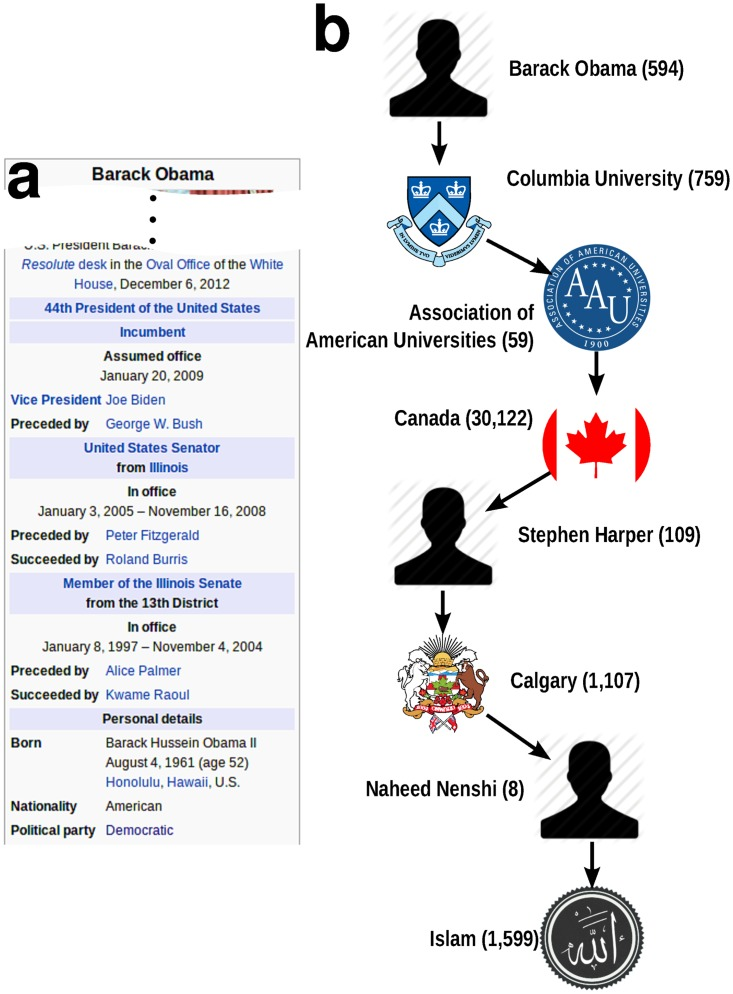
\includegraphics[width=0.5\linewidth]{img/barackObamaIsAMuslimNew.jpg}
	\caption{Wizualizacja zastosowania artykułów w\,Wikipedii do określenia prawdziwości stwierdzenia. źródło: \cite{ciampaglia2015computational}}
	\label{fig:barackObama}
\end{figure}
\par

\subsubsection{Context-based}
To podejście skupia się nie na treści prezentowanej informacji ale na jej kontekście. Jako kontekst można traktować autora tej informacji, serwis na którym się znajduje lub komentarze pozostawione przez odbiorców. Świetnym źródłem do zbierania tego typu informacji o kontekście są media społecznościowe. Ich idea polega na tym aby użytkownicy ingerowali w\,publikowane treści poprzez komentowanie, prowadzenie dyskusji i\,udostępnianie informacji większej grupie odbiorców.
\par
W obecnych czasach bardzo duże znaczenie mają media społecznościowe. Według badań z\,2018 roku 68\% ankietowanych pobiera wiedzę o aktualnych wydarzeniach właśnie z\,takich źródeł \cite{PewNewsUse2018}. Jest to wygodne i\,szybkie jednak bardzo podatne na manipulacje. Można jednak wykorzystać sieci zależności jakie tworzą źródła publikujące informacje z\,ich odbiorcami. Praca pod tytułem Some like it Hoax\cite{tacchini2017some} skupiła się na działalności użytkowników platformy Facebook jakim są ’polubienia’ postów. Projekt pobrał 15,500 postów polubionych przez ponad 900 tysięcy użytkowników. Aby wykrywać potencjalny fake news wykorzystał stworzony wcześniej podział stron na naukowe oraz o tematyce konspiracyjnej\cite{bessi2015science}. Wykorzystując fakt, że większość użytkowników ograniczała swoją aktywność tyko do postów należących do tylko jednej z\,tych kategorii, ale istnieje też niemała grupa akceptująca oba rodzaje stron możliwe było osiągnięcie bardzo wysokich wyników klasyfikacji postów do odpowiedniej kategorii. 
\par
Powstał również portal o nazwie Hoaxy\cite{shao2016hoaxy} na którym można prześledzić w\,formie grafu jak udostępniane są posty publikowane na Twitter. Dzięki tej aplikacji można zobaczyć, jak rozprzestrzenia się wskazany przez nas post, w\,czasie między kolejnymi użytkownikami. Przykład wykorzystania ukazano na rysunku \ref{fig:hoaxyTrump}. Znajduje się na nim wizualizacja sieci rozprzestrzeniania się wiadomości opublikowanej pierwotnie na koncie Donalda Trumpa dnia 03.05.2019. W\,czasie dwóch dni informacja ta została przekazana ponad 22 tysiące razy.
\begin{figure}[!h]
	
	\centering 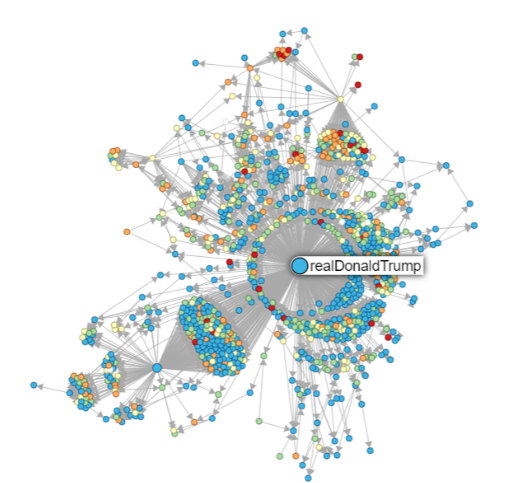
\includegraphics[width=0.5\linewidth]{img/hoaxy.png}
	\caption{Sieć rozprzestrzeniania się wiadomości na platformie Twitter na przykładzie wiadomości Donalda Trumpa. źródło: \url{https://hoaxy.iuni.iu.edu}}
	\label{fig:hoaxyTrump}
\end{figure}
\par
Innym podejściem do klasyfikacji źródeł publikujących informacje jest wykorzystanie odniesień jakie robią między sobą strony internetowe. Taką metodę wykorzystywał Pagerank działający dla Google. Wyznaczając rangę ważności strony brał on pod uwagę rangę stron, do których dana storna się odwoływała. Innym algorytmem wykorzystującą sieć skierowaną którą tworzą odniesienia jakie występują między stronami jest HITS. Opisuje on dwa typy stron: autorytety i\,koncentratory. Autorytetem jest strona, która jest często cytowana przez inne strony, natomiast koncentratorem jest strona, która wskazuje na wiele ważnych stron. Fakt, że strony internetowe zawierają odniesienia do innych stron można wykorzystać też do badania wiarygodności portali internetowych pod względem prawdziwości publikowanych informacji. Badania wykazały, że wykrywanie kłamliwych źródeł w\,takim grafie odbywa się z\,dużo większym sukcesem niż próba wykrycia tego przy zastosowaniu metod lingwistycznych bezpośrednio na publikowanych artykułach\cite{fairbanks2018credibility}. Wykorzystano w\,nich bazę danych pochodzącą z\,The Global Database o Events Language and Tone\footnote{\url{https://www.gdeltproject.org}}. Z\,pobranych artykułów podających linki zewnętrzne stworzono graf zawierający ponad 19 tysięcy unikalnych źródeł połączonych ponad 32 tysiącami linków. Oznaczenia wiarygodności dokonano na poziomie źródła, wykorzystano do tego istniejące oceny stron wykonane przez portal Media Bias Fact Check\footnote{\url{https://mediabiasfactcheck.com}}. Dzięki wykorzystaniu odpowiedniego algorytmu propagacji nie było wymagane, aby wszystkie źródła w\,grafie miały na wstępie zadeklarowaną ocenę. 
                                        % Wygodnie jest trzymać każdy rozdział w osobnym pliku.
%\newpage % Rozdziały zaczynamy od nowej strony.
\section{De Finibus Bonorum et Malorum}
Tu dam moj tekst.  Lorem ipsum dolor sit this is thext \footnote{This is footnote.}.
\begin{align*}
    E & = mc^2 \\
    y & = ax^2 + bx + c
\end{align*}

\lipsum[3]

\begin{align}
\begin{bmatrix}
    1 & 0 & 0 \\
    0 & 2 & 0 \\
    0 & 0 & 3
\end{bmatrix} \cdot
\begin{bmatrix}
    4 \\ 5 \\ 6
\end{bmatrix} =
\begin{bmatrix}
    4 \\ 10 \\ 18
\end{bmatrix}
\end{align}

\lipsum[4] Lorem ipsum dolor sit amet, consectetur adipiscing elit, sed do eiusmod tempor incididunt ut labore et dolore magna aliqua \cite{szczypiorski2015}, \cite{duqu2011}, \cite{shs2015}, \cite{wozniak2018}, \cite{dcp19}.

\subsection{Critique of Pure Reason}
\kant[1]

\begin{table}[!h] \label{tab:tabela1} \centering
\caption{Przykładowa tabela.}
\begin{tabular} {| c | c | r |} \hline
    Kolumna 1 & Kolumna 2 & Liczba \\ \hline\hline
    cell1 & cell2 & 60 \\ \hline
    cell4 & cell5 & 43 \\ \hline
    cell7 & cell8 & 20,45 \\ \hline
    \multicolumn{2}{|r|}{Suma:} & 123,45 \\ \hline
\end{tabular}
\end{table}

\kant[2]

\begin{longtable}{| c | m{0.58\linewidth} | r | m{0.1\linewidth} |}
    \caption{Tabela wielostronicowa.} \\
    \hline
    Lp & \multicolumn{1}{c|}{Treść} & \multicolumn{1}{c|}{Kwota} & \multicolumn{1}{m{0.1\linewidth}|}{Wariant opłaty} \\ \hline\hline \endfirsthead

    \endfoot
    \hline \endlastfoot

    1 & Lorem ipsum dolor sit amet, consectetur adipiscing elit, sed do eiusmod tempor incididunt ut labore et dolore magna aliqua. & 111 111,11 zł & \multicolumn{1}{c|}{WAR1} \\ \hline
    2 & Lorem ipsum dolor sit amet, consectetur adipiscing elit, sed do eiusmod tempor incididunt ut labore et dolore magna aliqua. & 22 222,22 zł & \multicolumn{1}{c|}{WAR1} \\ \hline
    3 & Lorem ipsum dolor sit amet, consectetur adipiscing elit, sed do eiusmod tempor incididunt ut labore et dolore magna aliqua. & 33 333,33 zł & \multicolumn{1}{c|}{WAR1} \\ \hline
    4 & Lorem ipsum dolor sit amet, consectetur adipiscing elit, sed do eiusmod tempor incididunt ut labore et dolore magna aliqua. & 444 444,44 zł & \multicolumn{1}{c|}{WAR1} \\ \hline
    5 & Lorem ipsum dolor sit amet, consectetur adipiscing elit, sed do eiusmod tempor incididunt ut labore et dolore magna aliqua. & 55 555,55 zł & \multicolumn{1}{c|}{WAR1} \\ \hline
    6 & Lorem ipsum dolor sit amet, consectetur adipiscing elit, sed do eiusmod tempor incididunt ut labore et dolore magna aliqua. & 66 666,66 zł & \multicolumn{1}{c|}{WAR1} \\ \hline
    7 & Lorem ipsum dolor sit amet, consectetur adipiscing elit, sed do eiusmod tempor incididunt ut labore et dolore magna aliqua. & 777 777,77 zł & \multicolumn{1}{c|}{WAR1} \\ \hline
    8 & Lorem ipsum dolor sit amet, consectetur adipiscing elit, sed do eiusmod tempor incididunt ut labore et dolore magna aliqua. & 8 888,88 zł & \multicolumn{1}{c|}{WAR1} \\ \hline
    9 & Lorem ipsum dolor sit amet, consectetur adipiscing elit, sed do eiusmod tempor incididunt ut labore et dolore magna aliqua. & 999 999,99 zł & \multicolumn{1}{c|}{WAR1} \\ \hline
    10 & Lorem ipsum dolor sit amet, consectetur adipiscing elit, sed do eiusmod tempor incididunt ut labore et dolore magna aliqua. & 111 111,11 zł & \multicolumn{1}{c|}{WAR2} \\ \hline
    11 & Lorem ipsum dolor sit amet, consectetur adipiscing elit, sed do eiusmod tempor incididunt ut labore et dolore magna aliqua. & 22 222,22 zł & \multicolumn{1}{c|}{WAR2} \\ \hline
    12 & Lorem ipsum dolor sit amet, consectetur adipiscing elit, sed do eiusmod tempor incididunt ut labore et dolore magna aliqua. & 33 333,33 zł & \multicolumn{1}{c|}{WAR2} \\ \hline
    13 & Lorem ipsum dolor sit amet, consectetur adipiscing elit, sed do eiusmod tempor incididunt ut labore et dolore magna aliqua. & 444 444,44 zł & \multicolumn{1}{c|}{WAR2} \\ \hline
    14 & Lorem ipsum dolor sit amet, consectetur adipiscing elit, sed do eiusmod tempor incididunt ut labore et dolore magna aliqua. & 55 555,55 zł & \multicolumn{1}{c|}{WAR2} \\ \hline
    15 & Lorem ipsum dolor sit amet, consectetur adipiscing elit, sed do eiusmod tempor incididunt ut labore et dolore magna aliqua. & 66 666,66 zł & \multicolumn{1}{c|}{WAR2} \\ \hline
    & \multicolumn{1}{r|}{\textbf{Suma:}} & \textbf{7 777 777,77 zł} &
    \label{table:koszty}
\end{longtable}
\kant[4]

\subsection{Categorical Imperative}
\subsubsection{Deontological Ethics}
As any dedicated reader can clearly see, the Ideal of practical reason is a representation of, as far as I know, the things in themselves; as I have shown elsewhere, the phenomena should only be used as a canon for our understanding:
% Parametr label ustawia symbol, a leftmargin - wielkość wcięcia.
% Domyślny układ to [---] bez wcięcia, bo tak pan Marcin Woliński powiedział;
% ale ja nie polecam. // AB
\begin{itemize}
    \item Item 1:
    \begin{itemize}[label=---]
        \item item 1.1;
        \item item 1.2;
        \item item 1.3;
    \end{itemize}
    \item Item 2;
    \item Item 3;
    \item Item 4.
\end{itemize}
\kant[2]

\subsubsection{Consequentialism -- the Ideal of practical reason}
\kant[3]
\begin{enumerate}
    \item Item 1:
    \begin{enumerate}
        \item item 1.1;
        \item item 1.2:
        \begin{enumerate}
            \item item 1.2.1;
            \item item 1.2.2;
        \end{enumerate}
        \item item 1.3;
    \end{enumerate}
    \item Item 2;
    \item Item 3;
    \item Item 4.
\end{enumerate}

\kant[9]

\subsection{G\"odel's ontological proof}
\kant[9] Lorem ipsum dolor sit amet, consectetur adipiscing elit, sed do eiusmod tempor incididunt ut labore et dolore magna aliqua \cite{benzmuller2014}, \cite{goedel95}, \cite{wang97}, \cite{koons2005}.
\begin{assumption} \label{ass:1}
    $ [\![ \ \phi \ ]\!] \Longrightarrow [\![ \ P(\phi); \neg P(\phi) \ ]\!]$
\end{assumption}
\begin{axiom}[Dualność] \label{axiom:1}
    $\neg P(\phi) \Leftrightarrow P(\neg \phi)$, równoważnie $P(\phi) \Leftrightarrow \neg P(\neg \phi)$
\end{axiom}
\begin{axiom}[Całkowitość] \label{axiom:2}
    $ \left( P(\phi) \wedge \forall x: \phi(x) \Rightarrow \psi(x) \right) \Rightarrow P(\psi) $
\end{axiom}
\begin{axiom}[Absolutność] \label{axiom:3}
    $ P(\phi) \Rightarrow \Box P(\phi) $
\end{axiom}
\begin{definition} \label{def:1}
    $ G(x) \Leftrightarrow \forall \phi: \left( P(\phi) \Rightarrow \phi(x) \right) $
\end{definition}
\begin{definition} \label{def:2}
    $ \phi \ ess \ x \Leftrightarrow \phi(x) \wedge \forall \psi \left( \psi(x) \Rightarrow \Box \forall y \left( \phi(y) \Rightarrow \psi(y) \right) \right)  $
\end{definition}
\begin{axiom} \label{axiom:4}
    P(G)
\end{axiom}
\begin{lemma} \label{lemma:1}
    $ P(\phi) \Rightarrow \Diamond \exists x : \phi(x) $
\end{lemma}
\begin{proof}
    Dowód pomijamy, bo jest trywialny :)
\end{proof}
\begin{lemma} \label{lemma:2}
    $ \Diamond \exists x : G(x) $
\end{lemma}
\begin{proof}
    Natychmiastowy wniosek z aksjomatu \ref{axiom:4} i lematu \ref{lemma:1}.
\end{proof}
\begin{lemma} \label{lemma:3}
    $ G(x) \Rightarrow G \ ess \ x $
\end{lemma}
\begin{proof}
    Poprzez podstawienie do definicji \ref{def:2}.
\end{proof}
\begin{definition} \label{def:3}
    $ E(x) \Leftrightarrow \forall \phi \left( \phi \ ess \ x \Rightarrow \Box\ \exists x: \phi(x) \right) $
\end{definition}
\begin{axiom} \label{axiom:5}
    P(E)
\end{axiom}
\begin{theorem}
    $ \Box\ \exists x : G(x) $
\end{theorem}
\begin{proof}
    Na podstawie definicji \ref{def:1}, lematu \ref{lemma:3} i aksjomatu \ref{axiom:5}.
\end{proof}    % Umożliwia to również łatwą migrację do nowej wersji szablonu:
%\newpage % Rozdziały zaczynamy od nowej strony.
\section{Code listings}

\lipsum[10]
% \addmargin pozwala na wcięcie kodu od lewej (tutaj: 6mm).
% Wcięcie pomaga ustawić kod tak, 
% aby numery linii nie były za bardzo na lewo. 
% Druga liczba oznacza wcięcie od prawej. 
\begin{addmargin}[6mm]{0mm}
\begin{lstlisting}[
    language=HTML,
    numbers=left,
    firstnumber=1,
    caption={\emph{Hello world} w HTML},
    aboveskip=0pt
]
<html>
  <head>
    <title>Hello world!</title>
  </head>
  <body>
    Hello world!
  </body>
</html>
\end{lstlisting}
\end{addmargin}

\lipsum[11]
% Dla dłuższych numerów linii
% potrzebne jest większe wcięcie.
\begin{addmargin}[10mm]{0mm}
\begin{lstlisting}[
    language=C++,
    numbers=left,
    firstnumber=147,
    caption={Generowanie sekwencji Collatza w języku C++},
    aboveskip=0pt
]
class Collatz {
  private:
    unsigned current_val_;
    void update_val() {
        if( current_val_ % 2 == 0 )
            current_val_ /= 2;
        else
            current_val_ = current_val_ * 3 + 1;
    }

  public:
    explicit Collatz(unsigned initial_value) : 
        current_val_(initial_value) {}
    void print_sequence() {
        unsigned i = 1;
        while( current_val_ > 1 ) {
            std::cout
                << "val " << i << " = " << current_val_
                << std::endl;
            update_val(); ++i;
        }
    }
};

int main() {
  // prints Collatz seqence, starting from 194375
  Collatz seq(194375);
  seq.print_sequence();
  return 0;
}
\end{lstlisting}
\end{addmargin}

\lipsum[12]
 % wystarczy podmienić swoje pliki main.tex i eiti-thesis.cls
                            % na nowe wersje, a cały tekst pracy pozostaje nienaruszony.

% \newpage % Rozdziały zaczynamy od nowej strony
% \section{Summatio}          % Można też pisać rozdziały w jednym pliku.
% \lipsum[5-10]

%--------------------------------------------
% Literatura
%--------------------------------------------
\cleardoublepage % Zaczynamy od nieparzystej strony
\printbibliography

%--------------------------------------------
% Spisy (opcjonalne)
%--------------------------------------------
\newpage
\pagestyle{plain}

% Wykaz symboli i skrótów.
% Pamiętaj, żeby posortować symbole alfabetycznie
% we własnym zakresie. Ponieważ mało kto używa takiego wykazu,
% uznałem, że robienie automatycznie sortowanej listy
% na poziomie LaTeXa to za duży overkill.
% Makro \acronymlist generuje właściwy tytuł sekcji,
% w zależności od języka.
% Makro \acronym dodaje skrót/symbol do listy,
% zapewniając podstawowe formatowanie.
% //AB
\vspace{0.8cm}
\acronymlist
\acronym{EiTI}{Wydział Elektroniki i Technik Informacyjnych}
\acronym{PW}{Politechnika Warszawska}
\acronym{WEIRD}{ang. \emph{Western, Educated, Industrialized, Rich and Democratic}}

\listoffigurestoc     % Spis rysunków.
\vspace{1cm}          % vertical space
\listoftablestoc      % Spis tabel.
\vspace{1cm}          % vertical space
\listofappendicestoc  % Spis załączników

% Załączniki
\newpage
\appendix{Nazwa załącznika 1}
\lipsum[1-8]

\newpage
\appendix{Nazwa załącznika 2}
\lipsum[1-4]

% Używając powyższych spisów jako szablonu,
% możesz tu dodać swój własny wykaz bądź listę,
% np. spis algorytmów.

\end{document} % Dobranoc.
